% Architektur
\chapter{Architektur Hochschul-App}
\label{sec:architektur}

Eine Anwendung, die täglich von einem Großteil der Studierenden der Hochschule Hof genutzt wird, bedarf einer gründlichen Vorbereitung in Bezug auf deren Umsetzung und Aufbau. Um den Anforderungen der Erweiterbarkeit, Langlebigkeit und der Modularität gerecht zu werden, sollte die grundlegende Architektur der Anwendung gründlich analysiert und erarbeitet werden. Anhand der Erkenntnisse, die in den vorigen Kapiteln erarbeitet wurden, wird im folgenden der Aufbau der Architektur der Hochschul-\ac{App} erläutert.

\section{Serviceorientierte Architektur}
\label{sec:arch_soa}

In Kapitel \ref{sec:ws_soa} \ac{SOA} wurden einige ausschlaggebende Argumente gebracht, die gezeigt haben, dass die Service-orientierte Architektur einen idealen Ansatz für die Umsetzung einer zukunftsfähigen Hochschul-\ac{App} mitbringt. Jedoch bringen Ser\-vice-orientierte Architekturen auch einige Nachteile mit sich. Anhand Abbildung \ref{fig:soaarch} kann man erkennen, welche Probleme bei einer Umsetzung der Datenschnittstelle der Hochschul-\ac{App} durch eine Service-orientierte Architektur auftreten können.

\begin{figure}[H]
\centering
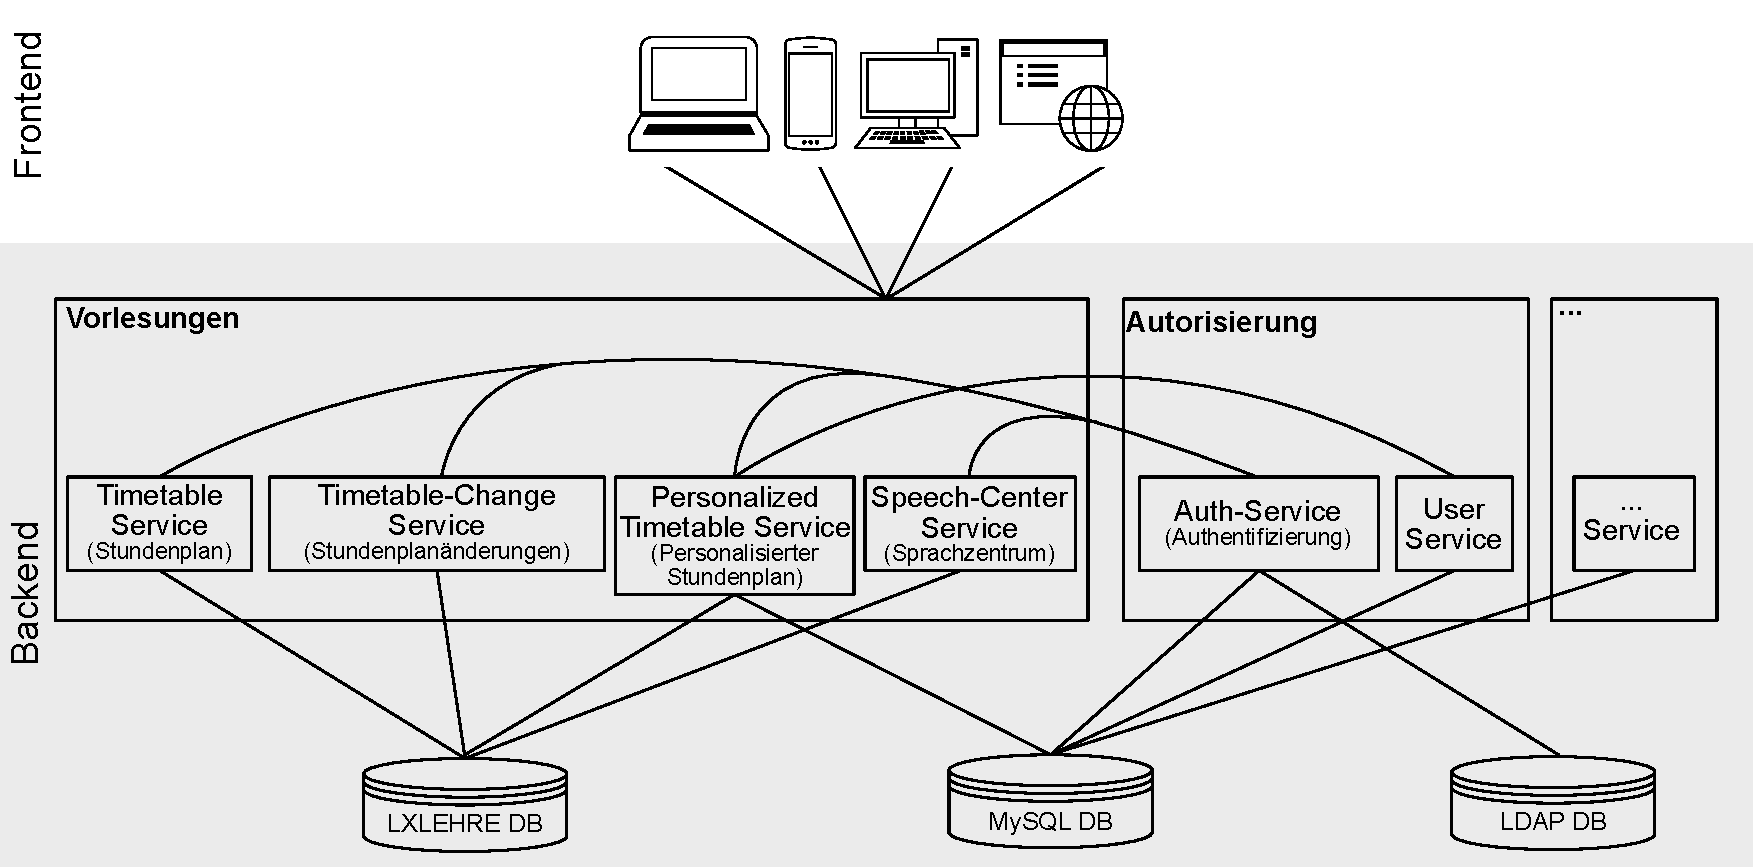
\includegraphics[,width=\pictureWidth cm + 2 cm]{Bilder/Architektur/SOA_FH_App_Architektur.pdf}
\caption{SOA Hochschul-App Architektur\label{fig:soaarch}\protect\footnotemark}
\end{figure}
\footnotetext{Brysiuk, Lehmann (2019)}


Zu erkennen ist einerseits, dass die Funktionalitäten der Anwendung in Services ausgelagert werden, die durch Module im Sourcecode getrennt sind und somit auch getrennt entwickelt werden können, jedoch nach dem Build-Prozess des Programmes in eine Komponente zusammengefasst werden. Die Entwicklung der Schnittstelle bleibt somit modular und flexibel, jedoch ist das Endprodukt nach jeder Änderung nach wie vor ein großer Monolith. Die Auslagerung und unabhängige Funktion der Services ist somit nicht gegeben, die Services können nicht nach deren Benutzungsstatistiken skaliert werden, lediglich die gesamte Anwendung könnte mehrmals parallel laufen, was aber weniger genutzte Teile der Anwendung ebenfalls hoch skalieren würde, was wiederum eine hohe Ressourcenverschwendung und hohe Kosten mit sich ziehen würde.
\\
\linebreak
Andererseits ist zu erkennen, das die Service-orientierte Architektur ebenfalls eine Abhängigkeit der einzelnen Services mit sich bringt. Bei einem Request müssen die Services Informationen untereinander austauschen können. So würde ein Request an den \textit{personalisierten Stundenplan} in der Service-orientierten Architektur die Folge haben, dass der Service zusätzlich Informationen vom \textit{User Service} benötigen würde um den Request verarbeiten zu können. Das erschafft Abhängigkeiten, durch die einzelne Services möglicherweise nicht mehr funktionieren, wenn sie benötigte Informationen nicht zurückerhalten. Außerdem ist zu erkennen, dass die Datenbank unter den Services geteilt wird. Durch die Verwendung einer gleicher Datenbank von mehreren Services könnten sogenannte \textit{Deadlocks} verursacht werden. Durch die bereits vorhandene Abhängigkeiten zwischen den Services wird die Ausfallwahrscheinlichkeit der Funktionalitäten durch diese \textit{Deadlocks} weiter verstärkt. Die Skalierung der Anwendung wird das Problem nicht lösen können, sondern im Gegenteil sogar verschlechtern, denn es entstehen immer mehr Instanzen die sich die gleichen Ressourcen teilen müssen.
\\
\linebreak
Um die Abhängigkeiten zu reduzieren und weitere vorhandene Probleme von \ac{SOA} zu minimieren steht der Microservice Architektur Ansatz zur Verfügung.
%Dieses Problem wird durch den Microservice Ansatz behoben, wodurch die Abhängigkeiten fast vollständig aufgelöst werden können.

\section{Microservice Architektur}

Die Microservice Architektur kann das Problem der Abhängigkeiten zwischen den Services bis zu einem gewissen Grat eliminieren. Im Beispiel des \textit{personalisierten Stundenplans} aus Kapitel \ref{sec:arch_soa} würden die benötigten Informationen aus dem \textit{User Service} lediglich als Übergabeparameter bei der Anfrage an den Service übergeben werden. Um dies genauer zu verstehen, werden die Grundlagen der Microservice Architektur im folgenden kurz erläutert.

\subsection*{Microservice Konzept}

Die Grundidee der Microservice Architektur kann durch das eben angebrachte Beispiel gut erklärt werden. In der \ac{SOA} Architektur werden die Funktionalitäten schon einmal in einzelne Module, Services genannt, getrennt. Diese sind jedoch nur im Entwicklungsprozess getrennt, nicht im Produktionsbetrieb, denn nach dem Build-Prozess und dem Deployment auf dem Server bilden diese Services einen einzigen Monolithen, der, wie schon in Kapitel \ref{sec:arch_soa} erwähnt wurde, nur im ganzen skaliert und vervielfacht werden kann. 
\\
\linebreak
Microservices lösen dieses Problem, in dem sie jeden Service nicht nur als Modul im Sourcecode trennen, sondern auch im Produktionsbetrieb. Jeder Service wird somit als eigene Anwendung gepflegt und kann unabhängig von allen anderen Services laufen und Anfragen bearbeiten. Die Vorteile dieser Strategie liegen auf der Hand.
\\
\linebreak
Zum einen können die einzelnen Services, in der Microservice Architektur auch Microservices genannt, einzeln skaliert werden. Somit können Teile der Anwendung, welche stark belastet werden, gut hoch skaliert werden, ohne auch die Teile der Anwendung zu skalieren, die kaum genutzt werden. Jeder Microservice kann als eigenes unabhängiges Modul auf unterschiedlichen Servern ausgelagert werden oder - wie bereits in Kapitel \ref{ws:zf} erwähnt wurde - in Cloud-basierte-Plattformen verschoben werden oder als Docker-Container realisiert werden. Somit können die vorhandenen Ressourcen optimal genutzt werden. Zum anderen kann man die Ausfallsicherheit und die Sicherheit im allgemeinen deutlich erhöhen, wenn man nur die einzelnen Microservices redundant hält. Sollte ein Microservice ausfallen, so kann eine andere Instanz des Services einsetzen, sollte keine weitere Instanz verfügbar sein, so läuft der Rest der Anwendung trotzdem problemlos weiter, da die anderen Funktionalitäten in eigene Microservices ausgelagert werden, die komplett unabhängig voneinander laufen. Somit werden durch die Microservice Architektur einige wichtige nicht-funktionale Anforderungen wie die Skalierbarkeit, Performance und Verfügbarkeit deutlich erweitert.  
\\
\linebreak
Aber auch \ac{DoS} und \ac{DDoS} Angriffe können einfacher kompensiert werden. Sollte keine Sicherheitsmaßnahme getroffen  werden, die solche Attacken frühzeitig erkennen, so würde bei einem Angriff auf einen einzelnen Microservice nur diese Funktionalität betroffen sein, die anderen Services, die unabhängig davon laufen, sind nicht gefährdet. Außerdem wird durch die erweiterte Modularisierung und Auflösung der Abhängigkeiten zwischen den Funktionalitäten das Testen, die Fehlerbehebung und die Erweiterungen der Funktionalitäten erleichtert. Die begründet sich einerseits, weil die Microservices leichtgewichtiger gestaltet sind, was die Erweiterbarkeit, Veränderbarkeit und Austauschbarkeit erleichtert, andererseits dadurch, dass durch die geringeren Abhängigkeiten die Komplexität der Funktionalitäten gemindert wird. Zusätzlich kann und sollte ebenfalls ein \ac{API}-Gateway genutzt werden, welches die Anfragen auf die einzelnen Microservices kontrolliert und nochmals eine Sicherheitsbarriere darstellt, sowie die einzelnen Microservices zu einer ganzen Anwendung verbindet. Wo diese in der Anwendung einzubinden ist, zeigt Abbildung \ref{fig:architektur_app}, genaueres zum \ac{API}-Gateway wird noch in Kapitel \ref{sec:api_gateway} erläutert. 

\begin{figure}[H]
\centering
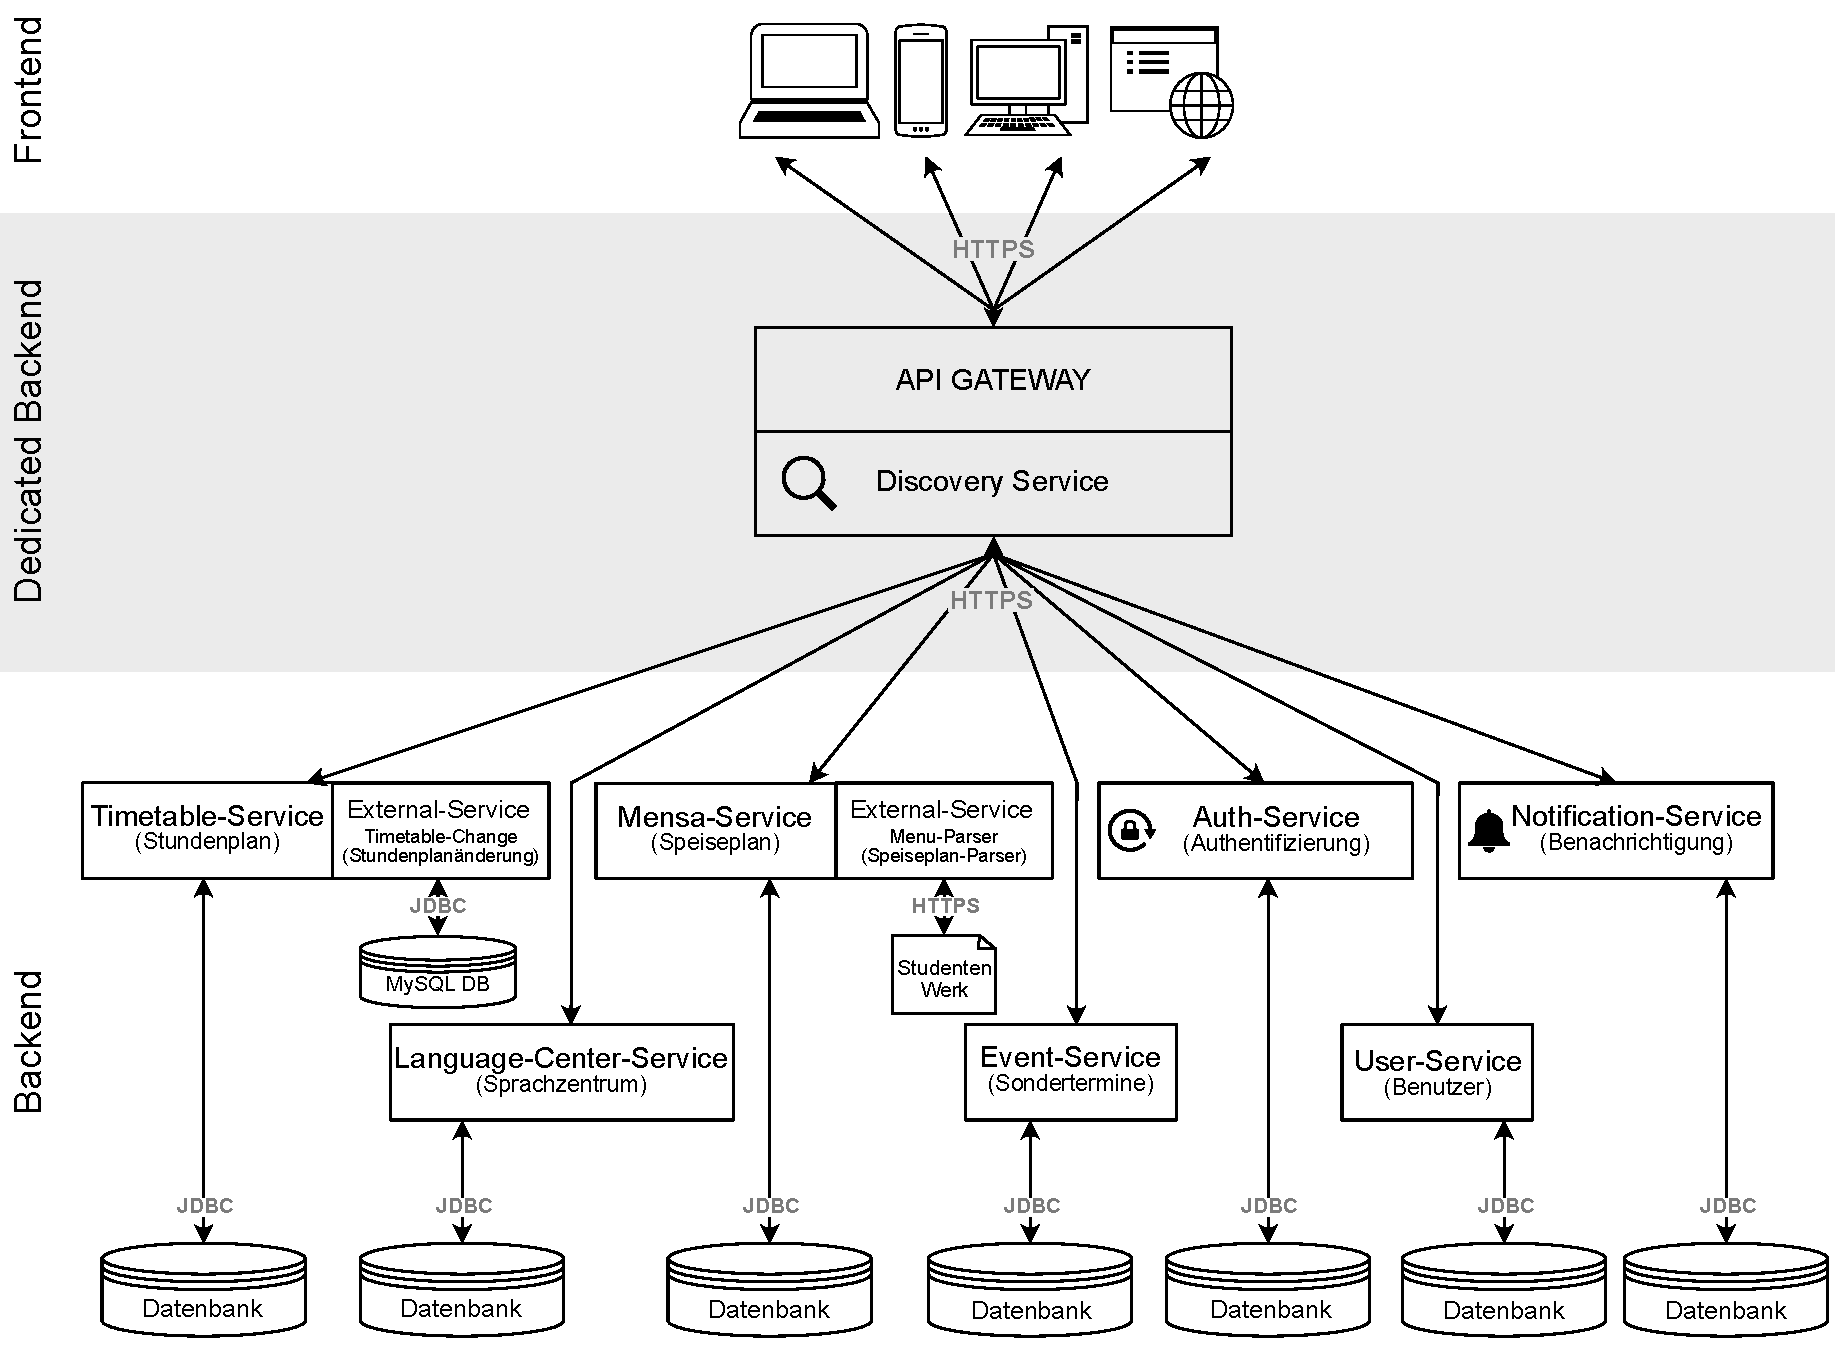
\includegraphics[,width=\pictureWidth cm + 2 cm]{Bilder/Architektur/MS_FH_App_Architektur.pdf}
\caption{Microservices Hochschul-App Architektur\label{fig:architektur_app}\protect\footnotemark}
\end{figure}
\footnotetext{Brysiuk, Lehmann (2019)}


Wie auf Abbildung \ref{fig:architektur_app} ebenfalls zu erkennen ist, wurden die einzelnen Anforderungen aus Kapitel \ref{sec:anforderung} in kleine unabhängige Microservices mit jeweils einer eigenen Datenbank getrennt. Das erfordert zwar, dass man mehrere Systeme aufsetzen muss, was mehr Aufwand in der Entwicklung bedeutet, jedoch kann man die Microservices und Datenbanken an die Bedürfnisse der einzelnen Funktionen anpassen und dementsprechend optimieren. So muss zum Beispiel nicht jeder Service auf die gleiche Art von Datenbank zurückgreifen, sonder kann die Art nutzen, die seine Anforderungen am besten erfüllt. Dies kann beispielsweise eine \ac{NoSQL}-Datenbank statt einer klassischen relationalen Datenbank sein, was bei einer \ac{SOA}-Architektur deutlich aufwändiger wäre, da dafür andere Schnittstellen in der Persistenz der Anwendung benötigt werden. Die Definition und die Spezifikation der einzelnen Microservices wird später noch in Kapitel \ref{sec:appservices} behandelt. 

\subsection*{Discovery Service\label{sec:discovery}}

Die Grundidee der Microservice Architektur zielt in großen Teilen auf die Skalierbarkeit und die gekapselte Zuständigkeit der einzelnen Services ab. Dieser Grundsatz beinhaltet im Wesentlichen zwei Teile. Einerseits möchte man bei der Kapselung der Zuständigkeiten der einzelnen Services erreichen, dass sowohl die Entwicklung, als auch der Produktionsbetrieb dieser Einzelteile unabhängig verlaufen können. Dabei spielen auch die physische Adresse und der Deployment-Server eine Rolle, denn einem Service, der gestartet wird, muss auch eine Adresse vergeben werden, mit er er angesprochen wird. Bei diesem Prozess spielt der \textit{Discovery Service} eine maßgebliche Rolle. Er bietet einen Anlaufpunkt, bei dem sich alle anderen Services mit ihrer Adresse registrieren können. Wird dann ein Service benötigt, so muss man den Discovery Service nur nach der Bezeichnung des Services fragen, worauf dieser dann mit der Adresse des gesuchten Services antwortet. 
\\
\linebreak
Andererseits möchte man bei der Aufteilung der Services erreichen, dass die einzelnen Instanzen optimal ausgelastet werden. So kann es bei der neuen Hochschul-Anwendung zum Beispiel vorkommen, dass der Stundenplan-Service stark ausgelastet ist, da das die zentrale Aufgabe dieser \ac{App} sein soll. Man kann bei Überlastungen dieses Services sehr einfach weitere Instanzen dessen auf anderen physikalischen Geräten deployen, um die Last gleichmäßig zu verteilen. Jedoch muss man nun einen Dienst einbinden, welcher die Adressen dieser Instanzen kennt und auch im Auge behält, welcher Dienst wie stark ausgelastet ist. Auch diese Aufgabe übernimmt der Discovery Service. Da sich alle Instanzen der Services mit ihrer Bezeichnung bei dem Discovery Service registrieren kann dieser die verschiedenen Instanzen des gleichen Services gruppieren und die Anfragen gleichmäßig verteilen. Der Client ruft dafür nur die Bezeichnung des Services beim Discovery Service ab und bekommt  darauf die Adresse des Services, der diese Aufgabe erledigt und der aktuell am wenigsten ausgelastet ist.
\\
\linebreak
Um diesen Discovery Service sinnvoll nutzen zu können, benötigt die Anwendung ein \ac{API}-Gateway, welches sich ebenfalls als Service beim Discovery Service registriert. Auch für dieses Gateway gilt, dass sich mehrere Instanzen registrieren können. Auch dieser Teil der Anwendung kann somit skaliert werden. Das \ac{API}-Gateway ruft dann für einen Client die Services beim Discovery Service ab. Die genaue Funktion des Gateways werden im Kapitel \ref{sec:api_gateway} \textit{API-Gateway} betrachtet. 

\subsection*{API-Gateway\label{sec:api_gateway}}

Als Verbindungsstück zwischen den Services und ihrer einzelnen Instanzen fungiert der im vorigen Kapitel \ref{sec:discovery} \textit{Discovery Service} beschriebene Service. Der große Vorteil dessen ist, dass man lediglich die Adresse des Discovery Services benötigt, um dann mit allen anderen Microservices zu kommunizieren. Um einem externen Client jedoch die Möglichkeit zu geben, die Vorteile dessen nutzen zu können, benötigt es ein \ac{API}-Gateway, bei dem der Nutzer die gewünschten Ressourcen anfragt und das sich dann um die Beschaffung dieser kümmert. Somit muss auch der Client nicht mehr jede Adresse der Services kennen, sondern nur die des\ac{API}-Gateways. Dies führt einerseits zu sauberem Code, da eine echte Adresse nicht mehr fest im Programmcode eingegeben werden muss, andererseits auch zu einer Möglichkeit, den Zugriff auf die Funktionen des Discovery Services und alle darunter liegenden Microservices zu kontrollieren.
\\
\linebreak
Die Funktion des \ac{API}-Gateways und der Zusammenarbeit des Discovery Services mit diesem werden in Abbildung \ref{fig:discovery_seq} gezeigt.

\begin{figure}[H]
\centering
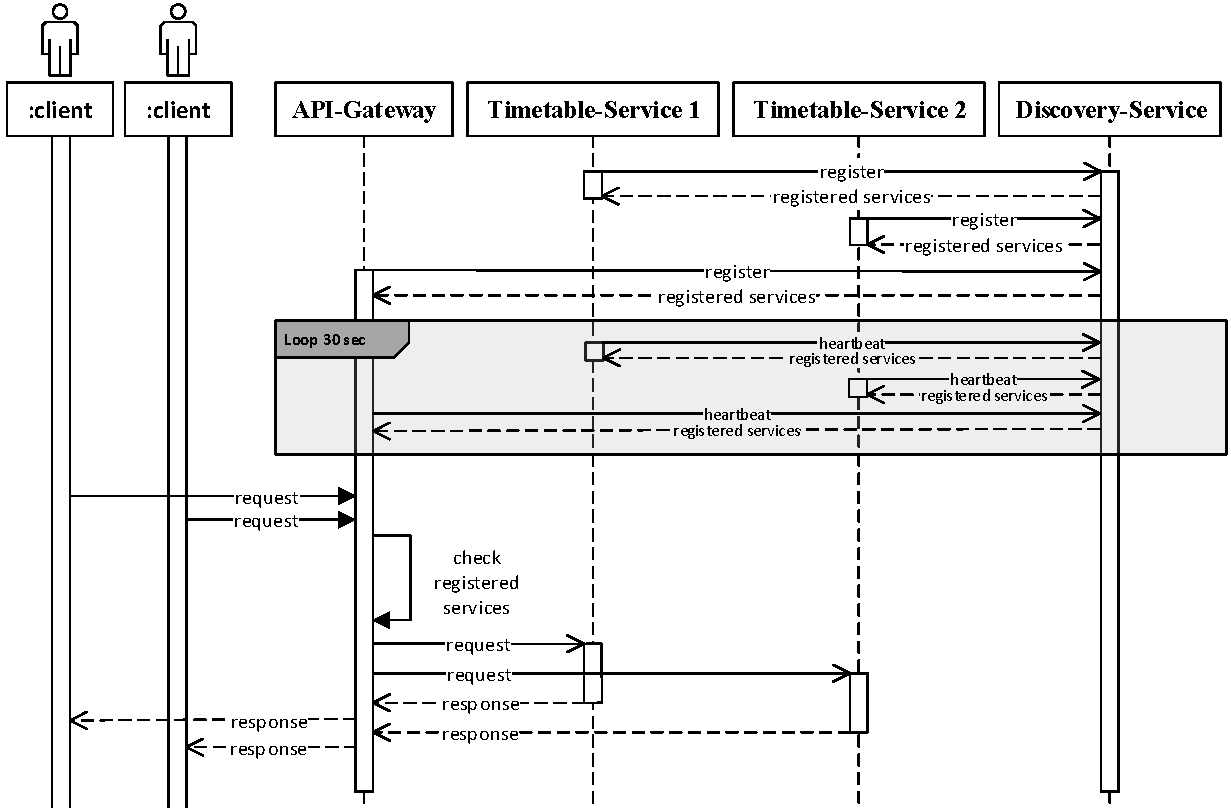
\includegraphics[,width=\pictureWidth cm + 2 cm]{Bilder/Sequenz_Diagramm/Discovery_Sequenz.pdf}
\caption{Sequenzdiagramm zwischen Discovery, \ac{API}-GATEWAY und Services\label{fig:discovery_seq}\protect\footnotemark}
\end{figure}
\footnotetext{Brysiuk, Lehmann (2019)}


Wie zu erkennen ist, registrieren sich alle Services, das \ac{API}-Gateway eingeschlossen, beim Discovery Service, welcher diesen dann eine Liste der aktuell registrierten Services und deren Adressen zurückgibt. Diese Liste wird in jedem Service gespeichert. Nach der erfolgreichen Registrierung melden sich die Services dann alle 30 Sekunden wieder beim Discovery Service, der dann wieder eine aktualisiert Liste zurückgibt. Dieses wiederholte Melden und Aktualisieren nennt man den \textit{Heartbeat} der registrierten Services. Sollte dieser Heartbeat einmal ausfallen, so entfernt der Discovery Service den Service, der sich nicht mehr meldet, automatisch nach einem definiertem Threshold an Fehlversuchen. 
\\
\linebreak
Sobald das \ac{API}-Gateway sich beim Discovery Service registriert hat, können die Clients erfolgreiche Anfragen an dieses schicken. Je nach Anfrage überprüft das Gateway dann, welcher passende Service bei ihm in der Liste, die er vom Discovery Service erhalten hat, enthalten ist und spricht diesen dann direkt mit der hinterlegten Adresse an. Die Antwort bekommt dieser darauf direkt vom angesprochenen Service, die Kommunikation läuft somit direkt zwischen den betroffenen Services, was die Performanz deutlich steigert. Lediglich die Registrierung und der Austausch der Adressen läuft parallel dazu im Hintergrund über den Discovery Service. 

\section{Schichtenarchitektur\label{sec:schichtenarchitektur}}

Wie bereit in Kapitel \ref{sec:layering} beschrieben wurde, soll die Architektur in Schichten aufgeteilt sein, um die Zuständigkeiten der einzelnen Funktionalitäten des Softwaresystems zu trennen und modular zu halten. Im Falle der Web-basierten Hochschul-\ac{App} trifft das auf die Architekturen der einzelnen Microservices zu. Diese werden, wie in Abbildung \ref{fig:ms_layer_alg} gezeigt, in 4 Schichten aufgeteilt, von denen eine nochmals physisch ausgelagert werden kann.

\begin{figure}[H]
\centering
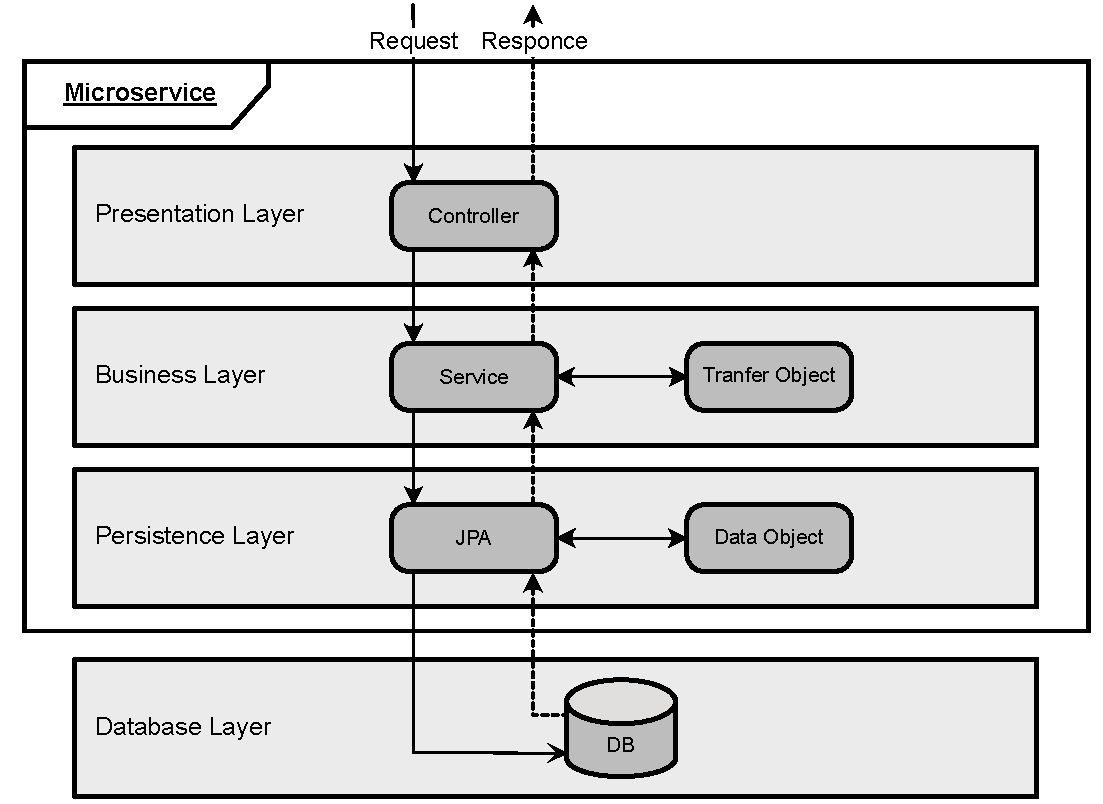
\includegraphics[,width=\pictureWidth cm]{Bilder/Architektur/MS_Schichtenarchitektur.pdf}
\caption{Microservice in Schichten Aufgeteilt\label{fig:ms_layer_alg}\protect\footnotemark}
\end{figure}
\footnotetext{Brysiuk, Lehmann (2019)}

Konkret übernehmen die Schichten folgende Aufgaben:

\begin{itemize}

\item \textbf{Presentation Layer} 
\\
Wie der Name der Schicht schon sagt, ist diese Schicht für die äußerliche Darstellung der Anwendung zuständig. Im Falle einer \ac{REST}-Schnittstelle sind das die Endpunkte, über die ein Client Daten abfragen kann. Diese Schicht ist nur für die Schnittstelle zuständig, sie definiert also die \acp{URL} für die Endpunkte und sichert die Anwendung nach außen ab. Zudem leitet sie die Anfragen an die darunterliegende Schicht, die Business Schicht, weiter.

\item \textbf{Business Layer} 
\\
Die Business Schicht übernimmt die eigentliche Aufgabe, für die die Anwendung geschrieben wurde. Sie enthält also die Kernlogik des Systems. Alle Algorithmen und Datenverarbeitungen werden in dieser Schicht durchgeführt. Benötigt eine dieser Vorgänge Daten, so werden diese aus der darunter liegenden Schicht, der Persistenz Schicht, abgefragt.

\item \textbf{Persistence Layer}
\\
Die Persistenz Schicht hat im Grunde nur zwei Aufgaben, Daten auszulesen und Daten zu speichern. Um die Datenquellen vor der Business Schicht zu verstecken und den Zugriff für alle Quellen zu vereinheitlichen bietet diese Schicht eine einheitliche Schnittstelle für die Daten aus allen Datenquellen. Wenn die Business Schicht die gelesenen Daten ändern möchte oder neue Daten einspeisen will, so kann sie das auch über die Persistenz Schicht tun. In diesem Fall gilt das gleiche Prinzip, wie beim Auslesen. Die Schnittstelle wird für alle Datenquellen angeglichen. So muss beim Austausch der Datenquellen nur die Persistenz Schicht, nie eine der darüber liegenden Schichten angepasst werden.

\item \textbf{Database Layer}
\\
Diese Schicht ist im Rahmen der Schichtenarchitektur nicht zwingend notwendig, allerdings wird sie im Großteil der Services der Hochschul-\ac{App} angewendet. Sie bildet die Grundlage der Datenschnittstelle der Services, die Datenbank. Die Datenbank ist kein Teil des eigentlichen Sourcecodes der Anwendung und kann somit separat zur Anwendung gepflegt werden. Jedoch kann die Anwendung ohne die Datenbank keine Daten bereitstellen, somit ist die Datenbank Schicht für die Hochschul-\ac{App} unverzichtbar.

\end{itemize}

\subsection*{Ablauf einer Anfrage}

Eine Anfrage eines Clients durchläuft im allgemeinen immer den selben Ablauf. Die Anfrage selbst wird an einen Endpunkt gerichtet, der durch eine \ac{URL} definiert wurde. Die Präsentations Schicht greift diese Anfrage auf und untersucht, ob der Client, der die Anfrage gestellt hat, die nötigen Berechtigungen für den Zugriff hat.
\\
\linebreak
Trifft das zu, so wird die Anfrage an die Business Schicht weitergeleitet, welche sie dann verarbeitet. Benötigt die Business Schicht zum Bearbeiten der Anfrage weitere Daten, so fragt sie diese in der Persistenz Schicht ab. Die Persistenz Schicht kann dann unterscheiden, um welche Art von Daten es sich handelt und wo diese zu finden sind. Sind die Daten aus der Datenbank auszulesen, so werden diese in der Datenbank Schicht abgefragt. Es kann sich aber auch um Daten handeln, welche von einem externen Anbieter geholt werden müssen. In diesem Fall schickt die Persistenz Schicht eine Anfrage an die Schnittstelle des externen Anbieters und liefert dann die Daten an die Business Schicht zurück. Die Daten werden zwischen der Persistenz Schicht und der Business Schicht immer in sogenannten \textit{Data Objects}, manchmal auch \textit{Business Entities} genannt, gekapselt. In der Programmiersprache Java werden diese Wrapper Objekte typischerweise mit dem Namen der Datenart, gefolgt von den Buchstaben \textit{\ac{DO}} benannt. 
\\
\linebreak
Die Business Schicht verarbeitet die Daten dann dementsprechend. Die veränderten Daten können dort auch wieder an die Persistenz Schicht weitergegeben werden, wo sie dann wieder in der zugehörigen Datenquelle abgespeichert werden. Im Falle der Hochschul-\ac{App} werden die Daten wieder in der Datenbank persistiert. Die Daten, die die Präsentations Schicht zur Beantwortung der Anfrage des Client benötigt, werden dann wieder von der Business Schicht an die Präsentations Schicht zurückgegeben. Diese Daten werden in \textit{Transfer Objects} weitergegeben. Hier werden die Wrapper Klassen in Java typischerweise mit dem Namen gefolgt von den Buchstaben \textit{\ac{TO}} benannt. 
\\
\linebreak
Die Antwort der Business Schicht an die Präsentations Schicht hängt immer von der Anfrage ab. Es können sowohl echte Daten, als auch nur Erfolgs-/ Misserfolgsbenachrichtigungen zurückgeliefert werden. Sollten Daten zurückgeliefert werden, so immer in Form von \textit{Transfer Objects}. Fehlermeldungen werden in in Java oft als Exceptions zurückgeliefert, in anderen Programmiersprachen mit ähnlichen Konstrukten. Erfolge werden meist durch Boolesche Werte oder durch das zurückkehren ohne Fehlermeldung signalisiert. Die empfangenen Rückgabewerte werden dann von der Präsentations Schicht an den Client zurückgegeben.
\\
\linebreak
Die Unterscheidung von \textit{Transfer Objects} und \textit{Data Objects} ist deshalb nötig, da in der Business Schicht oft Daten aus der Persistenz Schicht benötigt werden, die der Client entweder nicht einsehen darf, oder die er nicht verarbeiten kann. Deshalb werden die Daten, die über die Schnittstelle der Präsentations Schicht an den Client gehen, immer so bearbeitet, dass sie in der richtigen Form sind und keine sensiblen Daten mehr enthalten.

\subsection*{Aufbau der anwendungsinternen Schichten}

In Abbildung \ref{fig:ms_layer_alg} werden die groben Schichten der kompletten Software Architektur der Services und ihre Aufgaben betrachtet. Abbildung \ref{fig:ms_layer} hingegen betrachtet den Aufbau der drei oberen Schichten, die im Sourcecode der Anwendung liegen. Die Datenbank Schicht wird hierbei nicht weiter betrachtet. 

\subsubsection*{Package Struktur}

Ähnlich, wie die Schichten der Anwendung, wird auch der Programmcode unterteilt. Wie bereits in Kapitel \ref{sec:schichtenarchitektur} beschrieben wurde, sind die oberen drei Schichten auch im Sourcecode der Hochschul-\ac{App} zu finden. Die Package Struktur dieser richtet sich nach den drei Schichten, so gibt es ein Presentation Package, ein Business Package und ein Persistence Package. 
\\
\linebreak
Das Controller Package ist, wie zu erahnen ist, für die Endpunkte der Anwendung zuständig. In Microservice Anwendungen nennt man die zugehörigen Klassen oder Handler oft Controller, da es \ac{REST}-Schnittstellen sind, auch \ac{REST}-Controller. Demnach richtet sich auch die Namenskonvention. Den Anfang des Namens macht der Name der Schnittstelle, in Abbildung \ref{fig:ms_layer} beispielhaft \textit{Test} genannt, darauf folgend wird das Wort \textit{Controller} angehängt. Für jeden Teil der Schnittstelle kann man einen eigenen Controller definieren, so wird der Code auch übersichtlicher. 
\\
\linebreak
Das Service Package enthält alle Algorithmen zur Datenverarbeitung. Auch hier ist die Namenskonvention ähnlich wie im Controller Package aufgebaut, jedoch nennt man die zugehörigen Klassen oder Handler hier \textit{Services}. Der Namen beginnt auch hier mit dem Namen des Services und endet mit \textit{Service}. Zusätzlich zu den Services enthält dieses Package auch die in Kapitel \ref{sec:schichtenarchitektur} erwähnten \textit{Transfer Objects}. Diese werden im untergeordneten Package \textit{TransferObject} definiert. Die zugehörige Namenskonvention wurde bereits erläutert.
\\
\linebreak
Das letzte Package, das sich nach der allgemeinen Schichtenarchitektur richtet, ist das Repository Package. Hier werden die Daten aus den verschiedenen Datenquellen gesammelt. Die Namenskonvention ist hier unterschiedlich, je nachdem, um welche Art von Datenquelle es sich handelt. Bei nativen \ac{SQL}-Statements werden die zuständigen Klassen oder Handler oft \textit{DatabaseAccessor} oder \textit{[Name]Accessor} genannt. Bei externen Schnittstellen wird oft der Name gefolgt von der Abkürzung \textit{\ac{API}} genutzt. Bei der Nutzung der \ac{JPA} wir der Name der Datenquelle gefolgt von der Abkürzung \textit{\ac{JPA}} verwendet. Im Repository Package werden, wie in der Persistenz Schicht definiert wurde, auch die \textit{Data Objects} in einem untergeordneten Package gelagert. Auch für diese wurde die Namenskonvention bereits dargestellt. 
\\
\linebreak
Um die Aufgaben des Services von anderen Hilfsbibliotheken oder Prozeduren zu trennen benötigt die Package Struktur der Hochschul-\ac{App} und von Microservices im Allgemeinen noch weitere Packages für externes. Darunter gehören zum Beispiel externe Services, die man nicht ganz von der Aufgabe des Microservices trennen kann, die aber auch nicht direkt dazugehören. Ein Beispiel dafür ist der Zugriff auf eine externe Schnittstelle eines anderen Anbieters. Der Zugriff an sich wird dabei von einer externen Bibliothek durchgeführt. Ein weiteres Package ist das \textit{Util} Package. Dieses beinhaltet Hilfsbibliotheken und Klassen. Ein Beispiel hierfür sind Datenparser, welche gelesene Daten in ein einheitliches Format bringen.

\begin{figure}[H]
\centering
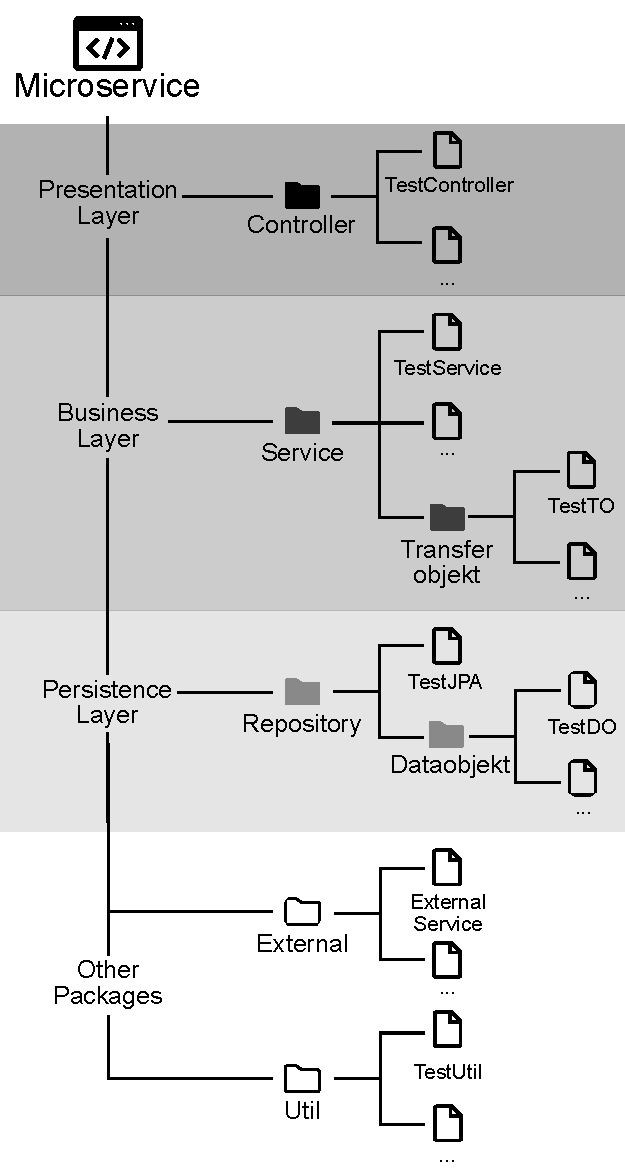
\includegraphics[,width=\pictureWidth cm -6 cm]{Bilder/Architektur/MS_Pakage_Stuktur.pdf}
\caption{Microservice Schichtenarchitektur\label{fig:ms_layer}\protect\footnotemark}
\end{figure}
\footnotetext{Brysiuk, Lehmann (2019)}

